\documentclass[12pt,letterpaper]{article}
\usepackage[margin=0.65in,top=0.72in,bottom=0.65in,headheight=17pt,headsep=14pt]{geometry}
\usepackage[T1]{fontenc}
\usepackage{helvet}
\renewcommand{\familydefault}{\sfdefault}
\usepackage{tikz}
\usetikzlibrary{arrows.meta}
\usepackage{fancyhdr}
\usepackage{array}
\pagestyle{fancy}
\fancyhf{}
\gdef\band{Grades 2--5}
\fancyhead[L]{\small Week 62 / Conflict networks / \band}
\fancyfoot[L]{\footnotesize Bellingham Math Circle / Week 62 / W62-S-v1}
\fancyfoot[R]{\footnotesize\thepage}
\renewcommand{\headrulewidth}{0.4pt}
\renewcommand{\footrulewidth}{0pt}
\setlength{\parindent}{0pt}
\setlength{\parskip}{7pt}
\newcommand{\recordline}[1]{\noindent #1\quad\rule{5in}{0.4pt}\par\vspace{0.35cm}}
\begin{document}
Each circle is one activity card. A line means its two cards cannot share a slot. Put every card in one slot. A slot can hold any number of cards if none of them conflict. Only marked circles are activities; line crossings add none. Write a card's slot number in its circle.

\begin{center}
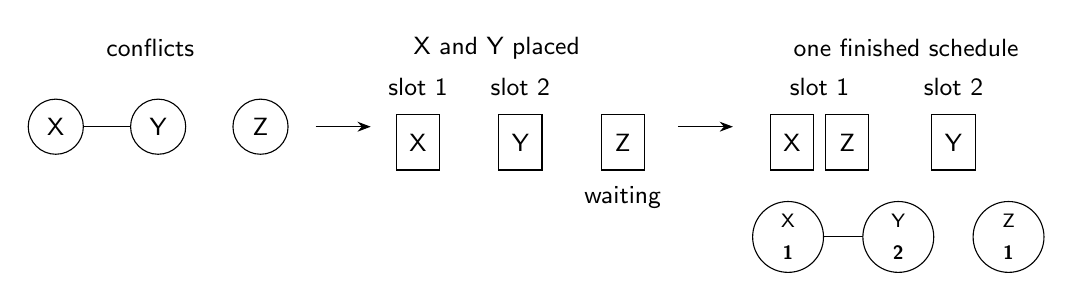
\begin{tikzpicture}[x=1cm,y=1cm,font=\small,card/.style={draw,minimum width=0.55cm,minimum height=0.7cm,fill=white},>=Stealth]
\node at (1.3,2) {conflicts};
\draw (0.1,1) -- (1.4,1);
\node[draw,circle,fill=white,minimum size=0.7cm] at (0.1,1) {X};
\node[draw,circle,fill=white,minimum size=0.7cm] at (1.4,1) {Y};
\node[draw,circle,fill=white,minimum size=0.7cm] at (2.7,1) {Z};
\draw[->] (3.4,1) -- (4.1,1);
\node at (5.7,2) {X and Y placed};
\node at (4.7,1.5) {slot 1}; \node[card] at (4.7,0.8) {X};
\node at (6,1.5) {slot 2}; \node[card] at (6,0.8) {Y};
\node[card] at (7.3,0.8) {Z}; \node at (7.3,0.1) {waiting};
\draw[->] (8,1) -- (8.7,1);
\node at (10.9,2) {one finished schedule};
\node at (9.8,1.5) {slot 1}; \node[card] at (9.45,0.8) {X}; \node[card] at (10.15,0.8) {Z};
\node at (11.5,1.5) {slot 2}; \node[card] at (11.5,0.8) {Y};
\draw (9.4,-0.4) -- (10.8,-0.4);
\foreach \x/\letter/\slot in {9.4/X/1,10.8/Y/2,12.2/Z/1}{
\node[draw,circle,fill=white,minimum size=0.9cm,inner sep=0pt] at (\x,-0.4) {};
\node[font=\scriptsize] at (\x,-0.2) {\letter};
\node[font=\scriptsize\bfseries] at (\x,-0.6) {\slot};
}
\end{tikzpicture}
\end{center}
\noindent\textbf{Problem 1:} Use your cards to schedule each network with the fewest slots you can.\par
\begin{center}
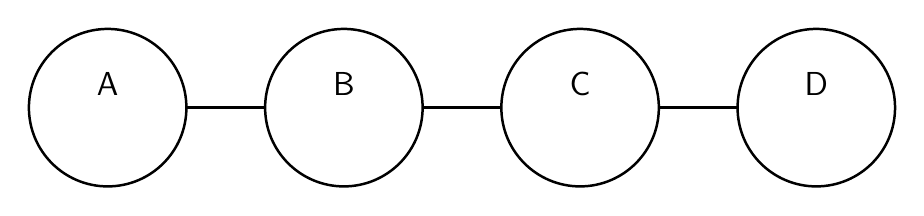
\begin{tikzpicture}[x=1cm,y=1cm,site/.style={circle,draw,line width=0.9pt,fill=white,minimum size=20mm,inner sep=0pt,font=\large},conflict/.style={line width=1.15pt}]
\coordinate (A) at (-4.5,1.5);
\coordinate (B) at (-1.5,1.5);
\coordinate (C) at (1.5,1.5);
\coordinate (D) at (4.5,1.5);
\draw[conflict] (A) -- (B);
\draw[conflict] (B) -- (C);
\draw[conflict] (C) -- (D);
\node[site] at (A) {};
\node[font=\large,yshift=3mm] at (A) {A};
\node[site] at (B) {};
\node[font=\large,yshift=3mm] at (B) {B};
\node[site] at (C) {};
\node[font=\large,yshift=3mm] at (C) {C};
\node[site] at (D) {};
\node[font=\large,yshift=3mm] at (D) {D};
\end{tikzpicture}
\end{center}
\begin{center}Fewest slots: \rule{1.1in}{0.4pt}\end{center}\begin{center}
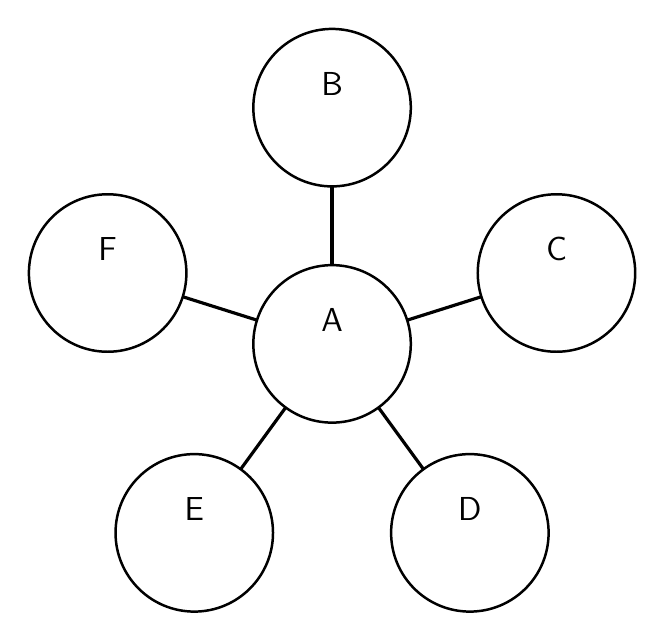
\begin{tikzpicture}[x=1cm,y=1cm,site/.style={circle,draw,line width=0.9pt,fill=white,minimum size=20mm,inner sep=0pt,font=\large},conflict/.style={line width=1.15pt}]
\coordinate (A) at (0,0);
\coordinate (B) at (0,3);
\coordinate (C) at (2.85,0.9);
\coordinate (D) at (1.75,-2.4);
\coordinate (E) at (-1.75,-2.4);
\coordinate (F) at (-2.85,0.9);
\draw[conflict] (A) -- (B);
\draw[conflict] (A) -- (C);
\draw[conflict] (A) -- (D);
\draw[conflict] (A) -- (E);
\draw[conflict] (A) -- (F);
\node[site] at (A) {};
\node[font=\large,yshift=3mm] at (A) {A};
\node[site] at (B) {};
\node[font=\large,yshift=3mm] at (B) {B};
\node[site] at (C) {};
\node[font=\large,yshift=3mm] at (C) {C};
\node[site] at (D) {};
\node[font=\large,yshift=3mm] at (D) {D};
\node[site] at (E) {};
\node[font=\large,yshift=3mm] at (E) {E};
\node[site] at (F) {};
\node[font=\large,yshift=3mm] at (F) {F};
\end{tikzpicture}
\end{center}
\begin{center}Fewest slots: \rule{1.1in}{0.4pt}\end{center}\clearpage\gdef\band{Grades 2--5}
\noindent\textbf{Problem 2:} Find the fewest slots for each network. Show why fewer slots cannot work.\par
\begin{center}\begin{minipage}[c]{0.48\linewidth}\centering
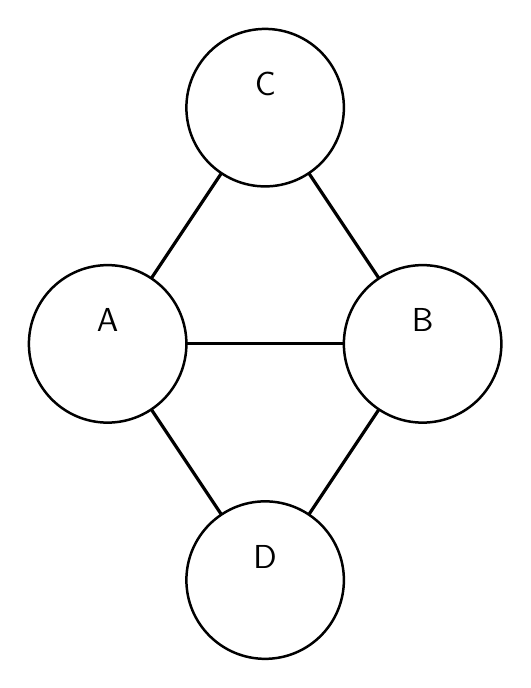
\begin{tikzpicture}[x=1cm,y=1cm,site/.style={circle,draw,line width=0.9pt,fill=white,minimum size=20mm,inner sep=0pt,font=\large},conflict/.style={line width=1.15pt}]
\coordinate (A) at (-2,0);
\coordinate (B) at (2,0);
\coordinate (C) at (0,3);
\coordinate (D) at (0,-3);
\draw[conflict] (A) -- (B);
\draw[conflict] (A) -- (C);
\draw[conflict] (B) -- (C);
\draw[conflict] (A) -- (D);
\draw[conflict] (B) -- (D);
\node[site] at (A) {};
\node[font=\large,yshift=3mm] at (A) {A};
\node[site] at (B) {};
\node[font=\large,yshift=3mm] at (B) {B};
\node[site] at (C) {};
\node[font=\large,yshift=3mm] at (C) {C};
\node[site] at (D) {};
\node[font=\large,yshift=3mm] at (D) {D};
\end{tikzpicture}\begin{center}Fewest slots: \rule{1.1in}{0.4pt}\end{center}\end{minipage}\hfill\begin{minipage}[c]{0.48\linewidth}\centering
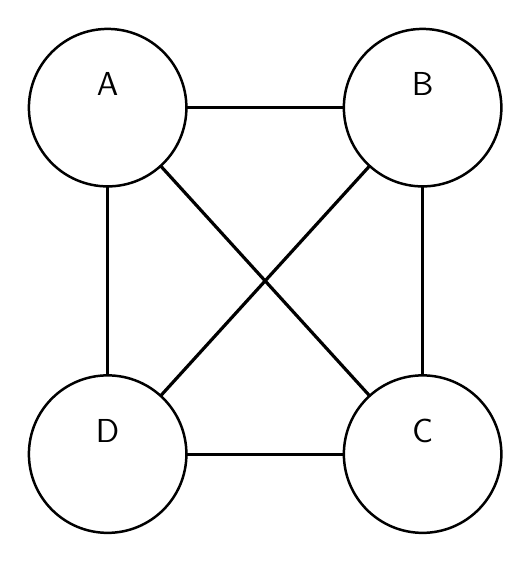
\begin{tikzpicture}[x=1cm,y=1cm,site/.style={circle,draw,line width=0.9pt,fill=white,minimum size=20mm,inner sep=0pt,font=\large},conflict/.style={line width=1.15pt}]
\coordinate (A) at (-2,2.2);
\coordinate (B) at (2,2.2);
\coordinate (C) at (2,-2.2);
\coordinate (D) at (-2,-2.2);
\draw[conflict] (A) -- (B);
\draw[conflict] (A) -- (C);
\draw[conflict] (A) -- (D);
\draw[conflict] (B) -- (C);
\draw[conflict] (B) -- (D);
\draw[conflict] (C) -- (D);
\node[site] at (A) {};
\node[font=\large,yshift=3mm] at (A) {A};
\node[site] at (B) {};
\node[font=\large,yshift=3mm] at (B) {B};
\node[site] at (C) {};
\node[font=\large,yshift=3mm] at (C) {C};
\node[site] at (D) {};
\node[font=\large,yshift=3mm] at (D) {D};
\end{tikzpicture}\begin{center}Fewest slots: \rule{1.1in}{0.4pt}\end{center}\end{minipage}\end{center}
\begin{center}
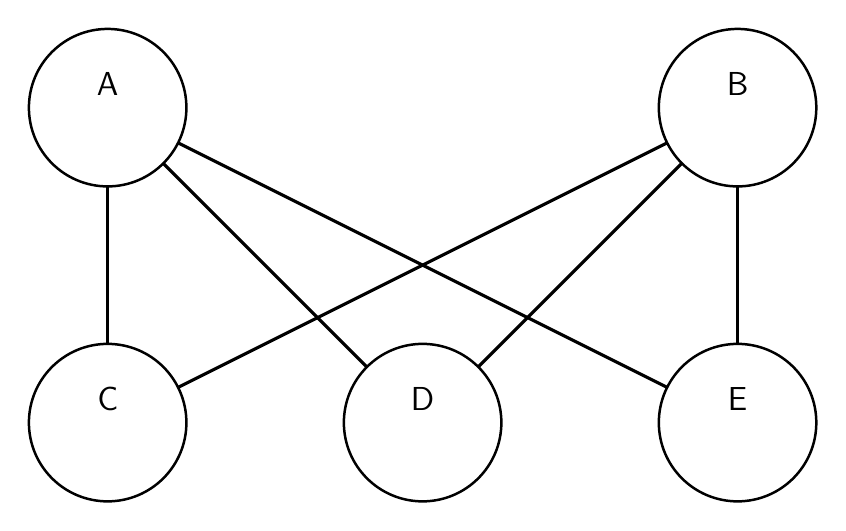
\begin{tikzpicture}[x=1cm,y=1cm,site/.style={circle,draw,line width=0.9pt,fill=white,minimum size=20mm,inner sep=0pt,font=\large},conflict/.style={line width=1.15pt}]
\coordinate (A) at (-4,2);
\coordinate (B) at (4,2);
\coordinate (C) at (-4,-2);
\coordinate (D) at (0,-2);
\coordinate (E) at (4,-2);
\draw[conflict] (A) -- (C);
\draw[conflict] (A) -- (D);
\draw[conflict] (A) -- (E);
\draw[conflict] (B) -- (C);
\draw[conflict] (B) -- (D);
\draw[conflict] (B) -- (E);
\node[site] at (A) {};
\node[font=\large,yshift=3mm] at (A) {A};
\node[site] at (B) {};
\node[font=\large,yshift=3mm] at (B) {B};
\node[site] at (C) {};
\node[font=\large,yshift=3mm] at (C) {C};
\node[site] at (D) {};
\node[font=\large,yshift=3mm] at (D) {D};
\node[site] at (E) {};
\node[font=\large,yshift=3mm] at (E) {E};
\end{tikzpicture}
\end{center}
\begin{center}Fewest slots: \rule{1.1in}{0.4pt}\end{center}\vspace{1cm}
\clearpage\gdef\band{Grades 2--5}
\noindent\textbf{Problem 3:} Find the fewest slots for each network. Also find the largest group of cards in which every pair conflicts. Does that group's size always give the fewest slots?\par
\begin{center}
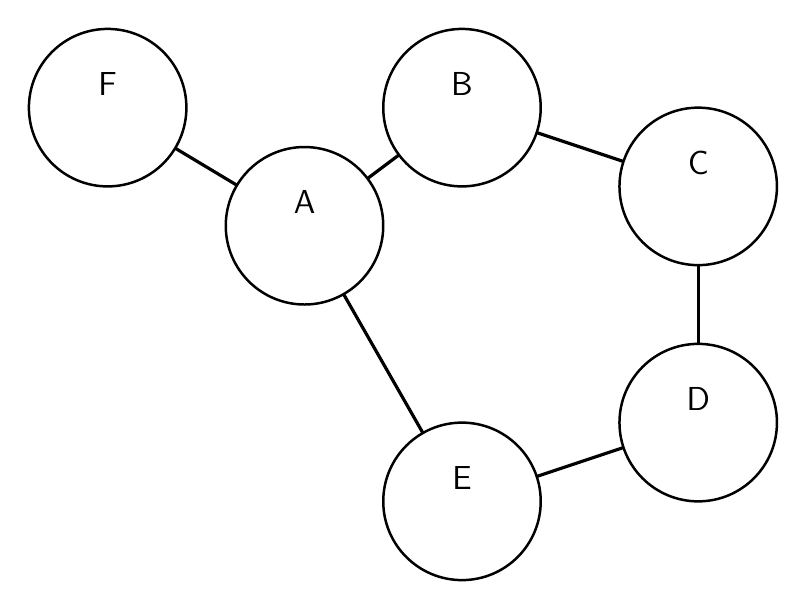
\begin{tikzpicture}[x=1cm,y=1cm,site/.style={circle,draw,line width=0.9pt,fill=white,minimum size=20mm,inner sep=0pt,font=\large},conflict/.style={line width=1.15pt}]
\coordinate (A) at (-3,1.5);
\coordinate (B) at (-1,3);
\coordinate (C) at (2,2);
\coordinate (D) at (2,-1);
\coordinate (E) at (-1,-2);
\coordinate (F) at (-5.5,3);
\draw[conflict] (A) -- (B);
\draw[conflict] (B) -- (C);
\draw[conflict] (C) -- (D);
\draw[conflict] (D) -- (E);
\draw[conflict] (E) -- (A);
\draw[conflict] (A) -- (F);
\node[site] at (A) {};
\node[font=\large,yshift=3mm] at (A) {A};
\node[site] at (B) {};
\node[font=\large,yshift=3mm] at (B) {B};
\node[site] at (C) {};
\node[font=\large,yshift=3mm] at (C) {C};
\node[site] at (D) {};
\node[font=\large,yshift=3mm] at (D) {D};
\node[site] at (E) {};
\node[font=\large,yshift=3mm] at (E) {E};
\node[site] at (F) {};
\node[font=\large,yshift=3mm] at (F) {F};
\end{tikzpicture}
\end{center}
\begin{center}Fewest slots: \rule{1.1in}{0.4pt}\end{center}\begin{center}
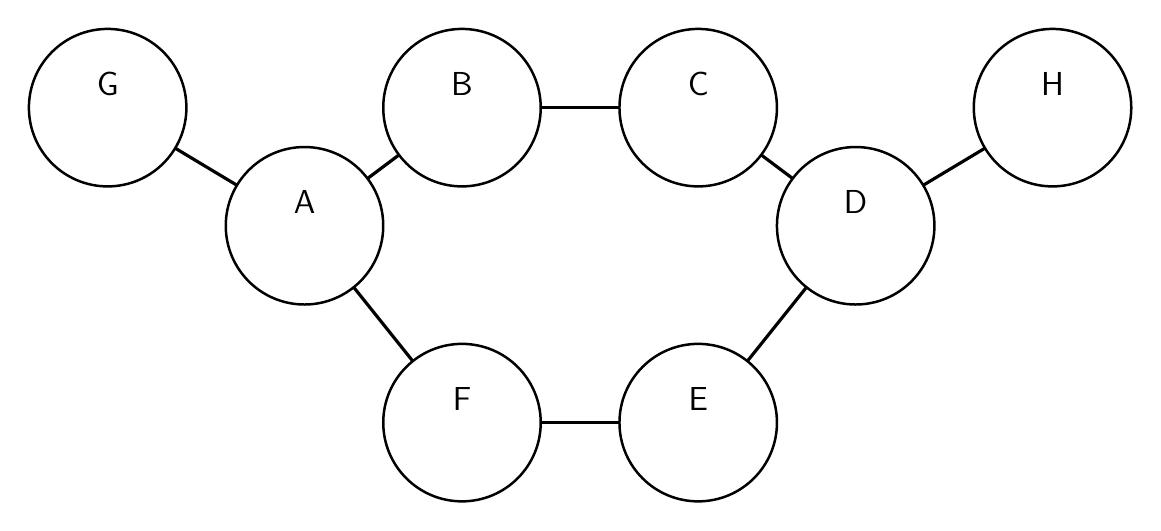
\begin{tikzpicture}[x=1cm,y=1cm,site/.style={circle,draw,line width=0.9pt,fill=white,minimum size=20mm,inner sep=0pt,font=\large},conflict/.style={line width=1.15pt}]
\coordinate (A) at (-3,1.5);
\coordinate (B) at (-1,3);
\coordinate (C) at (2,3);
\coordinate (D) at (4,1.5);
\coordinate (E) at (2,-1);
\coordinate (F) at (-1,-1);
\coordinate (G) at (-5.5,3);
\coordinate (H) at (6.5,3);
\draw[conflict] (A) -- (B);
\draw[conflict] (B) -- (C);
\draw[conflict] (C) -- (D);
\draw[conflict] (D) -- (E);
\draw[conflict] (E) -- (F);
\draw[conflict] (F) -- (A);
\draw[conflict] (A) -- (G);
\draw[conflict] (D) -- (H);
\node[site] at (A) {};
\node[font=\large,yshift=3mm] at (A) {A};
\node[site] at (B) {};
\node[font=\large,yshift=3mm] at (B) {B};
\node[site] at (C) {};
\node[font=\large,yshift=3mm] at (C) {C};
\node[site] at (D) {};
\node[font=\large,yshift=3mm] at (D) {D};
\node[site] at (E) {};
\node[font=\large,yshift=3mm] at (E) {E};
\node[site] at (F) {};
\node[font=\large,yshift=3mm] at (F) {F};
\node[site] at (G) {};
\node[font=\large,yshift=3mm] at (G) {G};
\node[site] at (H) {};
\node[font=\large,yshift=3mm] at (H) {H};
\end{tikzpicture}
\end{center}
\begin{center}Fewest slots: \rule{1.1in}{0.4pt}\end{center}\vspace{1cm}
\clearpage\gdef\band{Grades 4--5}
A cycle follows conflict lines through at least three different circles and back to its start. Only the start repeats, at the end.
\begin{center}
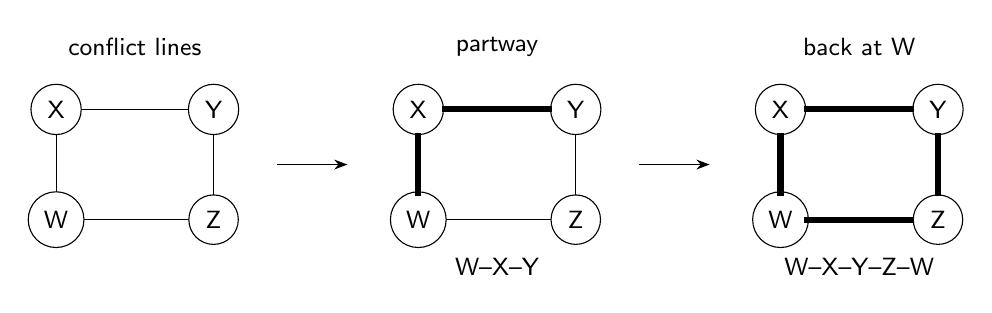
\begin{tikzpicture}[x=1cm,y=1cm,font=\small,>=Stealth]
\foreach \shift/\caption in {0/conflict lines,4.6/partway,9.2/back at W}{
\begin{scope}[shift={(\shift,0)}]
\node at (1,2.2) {\caption};
\draw (0,0) -- (0,1.4) -- (2,1.4) -- (2,0) -- cycle;
\node[draw,circle,fill=white,minimum size=0.55cm] at (0,0) {W};
\node[draw,circle,fill=white,minimum size=0.55cm] at (0,1.4) {X};
\node[draw,circle,fill=white,minimum size=0.55cm] at (2,1.4) {Y};
\node[draw,circle,fill=white,minimum size=0.55cm] at (2,0) {Z};
\end{scope}}
\draw[->] (2.8,0.7) -- (3.7,0.7); \draw[->] (7.4,0.7) -- (8.3,0.7);
\node at (5.6,-0.6) {W--X--Y}; \node at (10.2,-0.6) {W--X--Y--Z--W};
\draw[line width=2.2pt] (4.6,0.3) -- (4.6,1.1); \draw[line width=2.2pt] (4.9,1.4) -- (6.3,1.4);
\draw[line width=2.2pt] (9.2,0.3) -- (9.2,1.1); \draw[line width=2.2pt] (9.5,1.4) -- (10.9,1.4);
\draw[line width=2.2pt] (11.2,1.1) -- (11.2,0.3); \draw[line width=2.2pt] (10.9,0) -- (9.5,0);
\end{tikzpicture}
\end{center}
\noindent\textbf{Problem 4:} For each network, show a two-slot schedule if one exists. If it cannot fit in two slots, mark a cycle that explains why.\par
\begin{center}
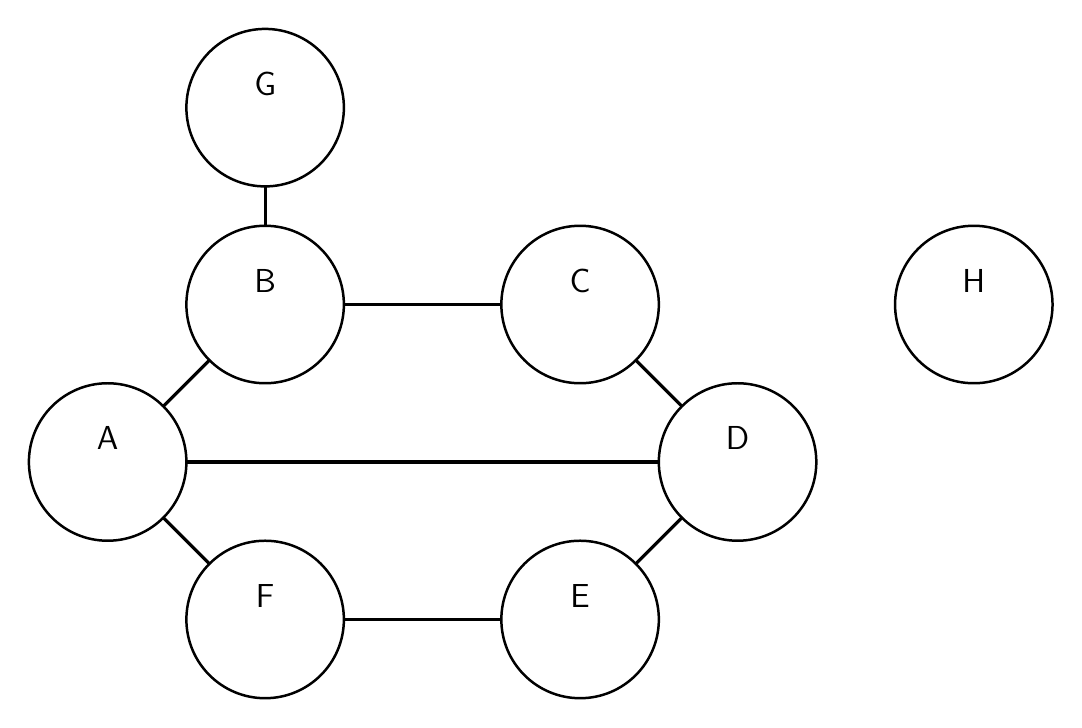
\begin{tikzpicture}[x=1cm,y=1cm,site/.style={circle,draw,line width=0.9pt,fill=white,minimum size=20mm,inner sep=0pt,font=\large},conflict/.style={line width=1.15pt}]
\coordinate (A) at (-4,1);
\coordinate (B) at (-2,3);
\coordinate (C) at (2,3);
\coordinate (D) at (4,1);
\coordinate (E) at (2,-1);
\coordinate (F) at (-2,-1);
\coordinate (G) at (-2,5.5);
\coordinate (H) at (7,3);
\draw[conflict] (A) -- (B);
\draw[conflict] (B) -- (C);
\draw[conflict] (C) -- (D);
\draw[conflict] (D) -- (E);
\draw[conflict] (E) -- (F);
\draw[conflict] (F) -- (A);
\draw[conflict] (A) -- (D);
\draw[conflict] (B) -- (G);
\node[site] at (A) {};
\node[font=\large,yshift=3mm] at (A) {A};
\node[site] at (B) {};
\node[font=\large,yshift=3mm] at (B) {B};
\node[site] at (C) {};
\node[font=\large,yshift=3mm] at (C) {C};
\node[site] at (D) {};
\node[font=\large,yshift=3mm] at (D) {D};
\node[site] at (E) {};
\node[font=\large,yshift=3mm] at (E) {E};
\node[site] at (F) {};
\node[font=\large,yshift=3mm] at (F) {F};
\node[site] at (G) {};
\node[font=\large,yshift=3mm] at (G) {G};
\node[site] at (H) {};
\node[font=\large,yshift=3mm] at (H) {H};
\end{tikzpicture}
\end{center}
\begin{center}
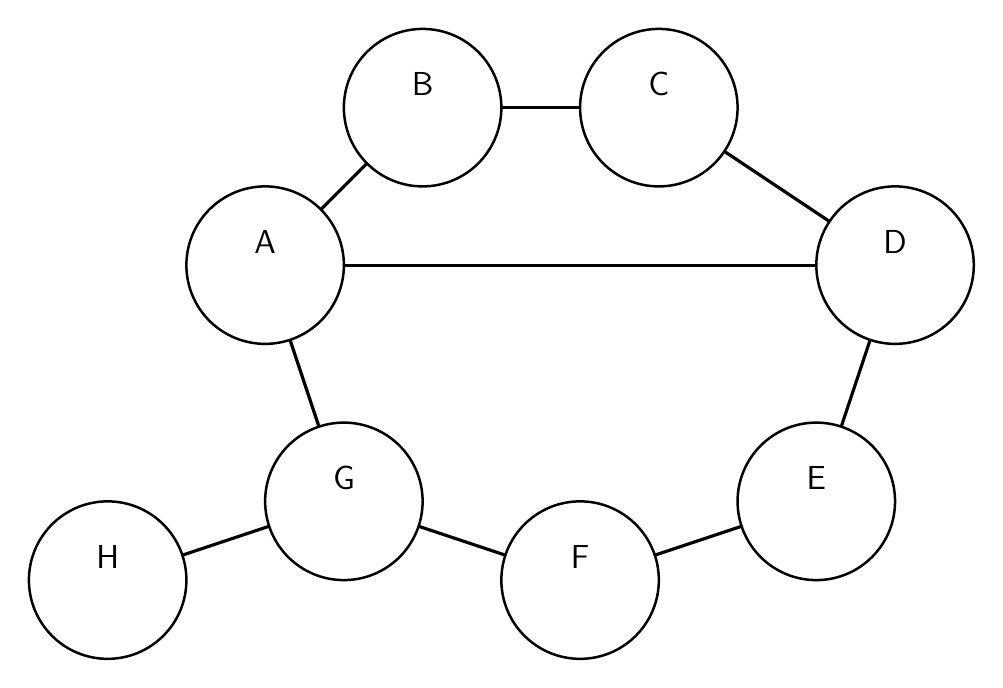
\begin{tikzpicture}[x=1cm,y=1cm,site/.style={circle,draw,line width=0.9pt,fill=white,minimum size=20mm,inner sep=0pt,font=\large},conflict/.style={line width=1.15pt}]
\coordinate (A) at (-4,1);
\coordinate (B) at (-2,3);
\coordinate (C) at (1,3);
\coordinate (D) at (4,1);
\coordinate (E) at (3,-2);
\coordinate (F) at (0,-3);
\coordinate (G) at (-3,-2);
\coordinate (H) at (-6,-3);
\draw[conflict] (A) -- (B);
\draw[conflict] (B) -- (C);
\draw[conflict] (C) -- (D);
\draw[conflict] (D) -- (E);
\draw[conflict] (E) -- (F);
\draw[conflict] (F) -- (G);
\draw[conflict] (G) -- (A);
\draw[conflict] (A) -- (D);
\draw[conflict] (G) -- (H);
\node[site] at (A) {};
\node[font=\large,yshift=3mm] at (A) {A};
\node[site] at (B) {};
\node[font=\large,yshift=3mm] at (B) {B};
\node[site] at (C) {};
\node[font=\large,yshift=3mm] at (C) {C};
\node[site] at (D) {};
\node[font=\large,yshift=3mm] at (D) {D};
\node[site] at (E) {};
\node[font=\large,yshift=3mm] at (E) {E};
\node[site] at (F) {};
\node[font=\large,yshift=3mm] at (F) {F};
\node[site] at (G) {};
\node[font=\large,yshift=3mm] at (G) {G};
\node[site] at (H) {};
\node[font=\large,yshift=3mm] at (H) {H};
\end{tikzpicture}
\end{center}
\clearpage\gdef\band{Grades 4--5}
\noindent\textbf{Problem 5:} Make a rule that decides which networks fit in two slots. Use it on these networks. Explain why your rule works for networks of any size.\par
\begin{center}
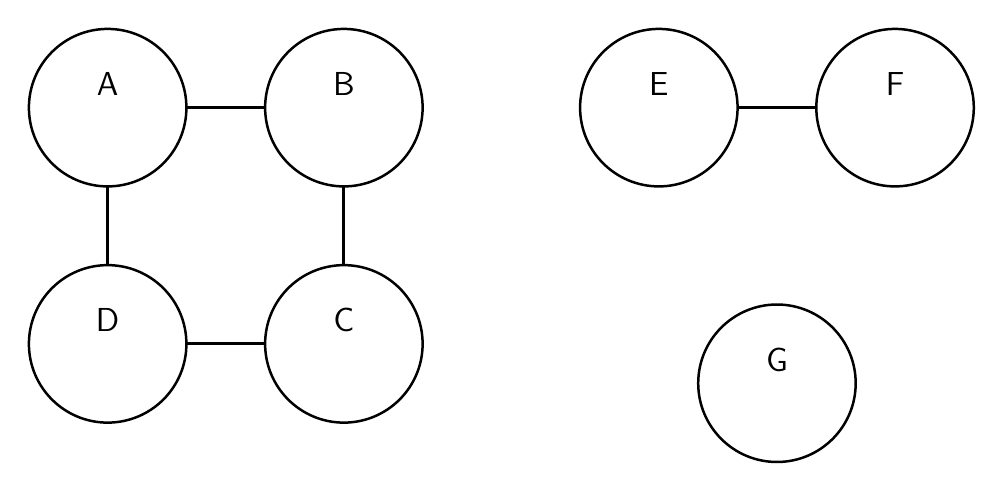
\begin{tikzpicture}[x=1cm,y=1cm,site/.style={circle,draw,line width=0.9pt,fill=white,minimum size=20mm,inner sep=0pt,font=\large},conflict/.style={line width=1.15pt}]
\coordinate (A) at (-5,2);
\coordinate (B) at (-2,2);
\coordinate (C) at (-2,-1);
\coordinate (D) at (-5,-1);
\coordinate (E) at (2,2);
\coordinate (F) at (5,2);
\coordinate (G) at (3.5,-1.5);
\draw[conflict] (A) -- (B);
\draw[conflict] (B) -- (C);
\draw[conflict] (C) -- (D);
\draw[conflict] (D) -- (A);
\draw[conflict] (E) -- (F);
\node[site] at (A) {};
\node[font=\large,yshift=3mm] at (A) {A};
\node[site] at (B) {};
\node[font=\large,yshift=3mm] at (B) {B};
\node[site] at (C) {};
\node[font=\large,yshift=3mm] at (C) {C};
\node[site] at (D) {};
\node[font=\large,yshift=3mm] at (D) {D};
\node[site] at (E) {};
\node[font=\large,yshift=3mm] at (E) {E};
\node[site] at (F) {};
\node[font=\large,yshift=3mm] at (F) {F};
\node[site] at (G) {};
\node[font=\large,yshift=3mm] at (G) {G};
\end{tikzpicture}
\end{center}
\begin{center}
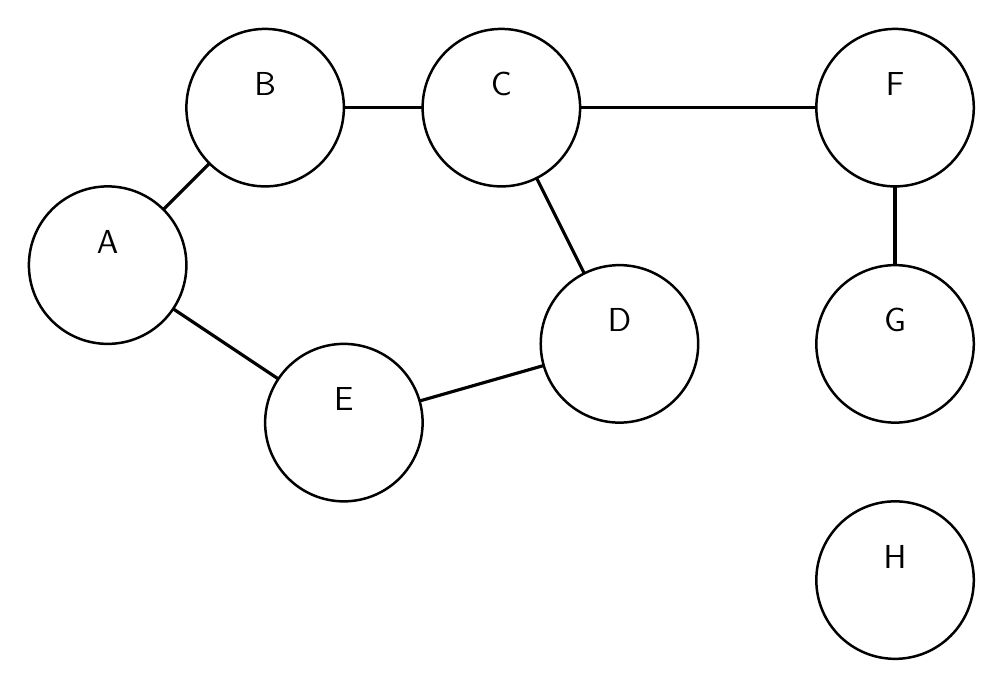
\begin{tikzpicture}[x=1cm,y=1cm,site/.style={circle,draw,line width=0.9pt,fill=white,minimum size=20mm,inner sep=0pt,font=\large},conflict/.style={line width=1.15pt}]
\coordinate (A) at (-5,1);
\coordinate (B) at (-3,3);
\coordinate (C) at (0,3);
\coordinate (D) at (1.5,0);
\coordinate (E) at (-2,-1);
\coordinate (F) at (5,3);
\coordinate (G) at (5,0);
\coordinate (H) at (5,-3);
\draw[conflict] (A) -- (B);
\draw[conflict] (B) -- (C);
\draw[conflict] (C) -- (D);
\draw[conflict] (D) -- (E);
\draw[conflict] (E) -- (A);
\draw[conflict] (C) -- (F);
\draw[conflict] (F) -- (G);
\node[site] at (A) {};
\node[font=\large,yshift=3mm] at (A) {A};
\node[site] at (B) {};
\node[font=\large,yshift=3mm] at (B) {B};
\node[site] at (C) {};
\node[font=\large,yshift=3mm] at (C) {C};
\node[site] at (D) {};
\node[font=\large,yshift=3mm] at (D) {D};
\node[site] at (E) {};
\node[font=\large,yshift=3mm] at (E) {E};
\node[site] at (F) {};
\node[font=\large,yshift=3mm] at (F) {F};
\node[site] at (G) {};
\node[font=\large,yshift=3mm] at (G) {G};
\node[site] at (H) {};
\node[font=\large,yshift=3mm] at (H) {H};
\end{tikzpicture}
\end{center}
\vspace{0.5cm}
\noindent My rule:\quad\rule{5.7in}{0.4pt}\par\vspace{0.7cm}\hrule\vspace{0.9cm}\hrule
\clearpage\gdef\band{Grades 4--5}
\noindent\textbf{Problem 6:} Add the fewest conflict lines you can so each network can no longer fit in two slots. Join only different circles that have no line yet. Show why fewer added lines cannot work.\par
\begin{center}
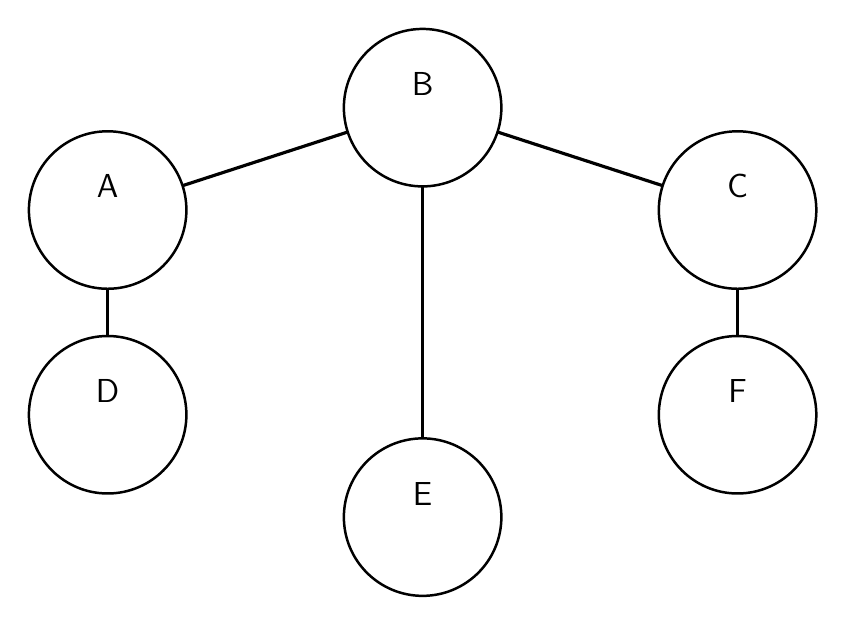
\begin{tikzpicture}[x=1cm,y=1cm,site/.style={circle,draw,line width=0.9pt,fill=white,minimum size=20mm,inner sep=0pt,font=\large},conflict/.style={line width=1.15pt}]
\coordinate (A) at (-4,1.3);
\coordinate (B) at (0,2.6);
\coordinate (C) at (4,1.3);
\coordinate (D) at (-4,-1.3);
\coordinate (E) at (0,-2.6);
\coordinate (F) at (4,-1.3);
\draw[conflict] (A) -- (B);
\draw[conflict] (B) -- (C);
\draw[conflict] (A) -- (D);
\draw[conflict] (B) -- (E);
\draw[conflict] (C) -- (F);
\node[site] at (A) {};
\node[font=\large,yshift=3mm] at (A) {A};
\node[site] at (B) {};
\node[font=\large,yshift=3mm] at (B) {B};
\node[site] at (C) {};
\node[font=\large,yshift=3mm] at (C) {C};
\node[site] at (D) {};
\node[font=\large,yshift=3mm] at (D) {D};
\node[site] at (E) {};
\node[font=\large,yshift=3mm] at (E) {E};
\node[site] at (F) {};
\node[font=\large,yshift=3mm] at (F) {F};
\end{tikzpicture}
\end{center}
\begin{center}Added lines: \rule{1.2in}{0.4pt}\end{center}
\begin{center}
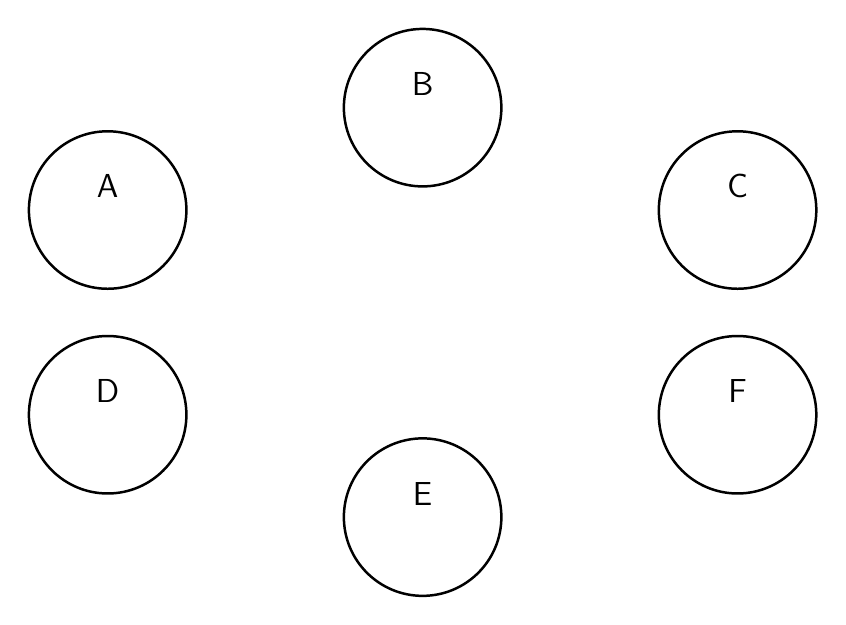
\begin{tikzpicture}[x=1cm,y=1cm,site/.style={circle,draw,line width=0.9pt,fill=white,minimum size=20mm,inner sep=0pt,font=\large},conflict/.style={line width=1.15pt}]
\coordinate (A) at (-4,1.3);
\coordinate (B) at (0,2.6);
\coordinate (C) at (4,1.3);
\coordinate (D) at (-4,-1.3);
\coordinate (E) at (0,-2.6);
\coordinate (F) at (4,-1.3);
\node[site] at (A) {};
\node[font=\large,yshift=3mm] at (A) {A};
\node[site] at (B) {};
\node[font=\large,yshift=3mm] at (B) {B};
\node[site] at (C) {};
\node[font=\large,yshift=3mm] at (C) {C};
\node[site] at (D) {};
\node[font=\large,yshift=3mm] at (D) {D};
\node[site] at (E) {};
\node[font=\large,yshift=3mm] at (E) {E};
\node[site] at (F) {};
\node[font=\large,yshift=3mm] at (F) {F};
\end{tikzpicture}
\end{center}
\begin{center}Added lines: \rule{1.2in}{0.4pt}\end{center}\vspace{1.6cm}
\clearpage\gdef\band{Grades 4--5}
For Problems 7--8, choose an order for the cards. Place each card in the first numbered slot where it conflicts with no card already there. During the order, do not move a placed card.
\begin{center}
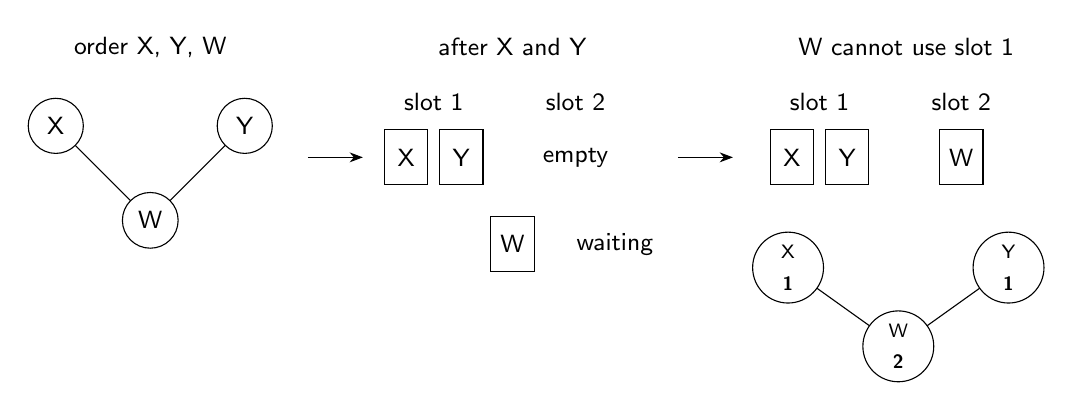
\begin{tikzpicture}[x=1cm,y=1cm,font=\small,card/.style={draw,minimum width=0.55cm,minimum height=0.7cm,fill=white},>=Stealth]
\node at (1.3,2.7) {order X, Y, W};
\draw (0.1,1.7) -- (1.3,0.5) -- (2.5,1.7);
\node[draw,circle,fill=white,minimum size=0.7cm] at (0.1,1.7) {X};
\node[draw,circle,fill=white,minimum size=0.7cm] at (2.5,1.7) {Y};
\node[draw,circle,fill=white,minimum size=0.7cm] at (1.3,0.5) {W};
\draw[->] (3.3,1.3) -- (4,1.3);
\node at (5.9,2.7) {after X and Y};
\node at (4.9,2) {slot 1}; \node[card] at (4.55,1.3) {X}; \node[card] at (5.25,1.3) {Y};
\node at (6.7,2) {slot 2}; \node at (6.7,1.3) {empty};
\node[card] at (5.9,0.2) {W}; \node at (7.2,0.2) {waiting};
\draw[->] (8,1.3) -- (8.7,1.3);
\node at (10.9,2.7) {W cannot use slot 1};
\node at (9.8,2) {slot 1}; \node[card] at (9.45,1.3) {X}; \node[card] at (10.15,1.3) {Y};
\node at (11.6,2) {slot 2}; \node[card] at (11.6,1.3) {W};
\draw (9.4,-0.1) -- (10.8,-1.1) -- (12.2,-0.1);
\foreach \x/\y/\letter/\slot in {9.4/-0.1/X/1,12.2/-0.1/Y/1,10.8/-1.1/W/2}{
\node[draw,circle,fill=white,minimum size=0.9cm,inner sep=0pt] at (\x,\y) {};
\node[font=\scriptsize,yshift=2mm] at (\x,\y) {\letter};
\node[font=\scriptsize\bfseries,yshift=-2mm] at (\x,\y) {\slot};
}
\end{tikzpicture}
\end{center}
\noindent\textbf{Problem 7:} Find orders that make the rule use as few slots and as many slots as possible on this network. After an order is finished, you may move cards. Can you use fewer slots?\par
\begin{center}
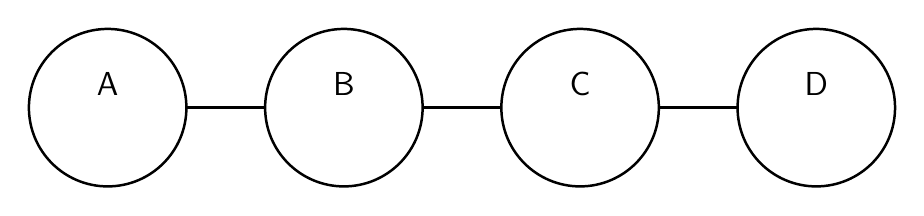
\begin{tikzpicture}[x=1cm,y=1cm,site/.style={circle,draw,line width=0.9pt,fill=white,minimum size=20mm,inner sep=0pt,font=\large},conflict/.style={line width=1.15pt}]
\coordinate (A) at (-4.5,1.5);
\coordinate (B) at (-1.5,1.5);
\coordinate (C) at (1.5,1.5);
\coordinate (D) at (4.5,1.5);
\draw[conflict] (A) -- (B);
\draw[conflict] (B) -- (C);
\draw[conflict] (C) -- (D);
\node[site] at (A) {};
\node[font=\large,yshift=3mm] at (A) {A};
\node[site] at (B) {};
\node[font=\large,yshift=3mm] at (B) {B};
\node[site] at (C) {};
\node[font=\large,yshift=3mm] at (C) {C};
\node[site] at (D) {};
\node[font=\large,yshift=3mm] at (D) {D};
\end{tikzpicture}
\end{center}
\recordline{Order:}\vspace{0.25cm}
\begin{center}
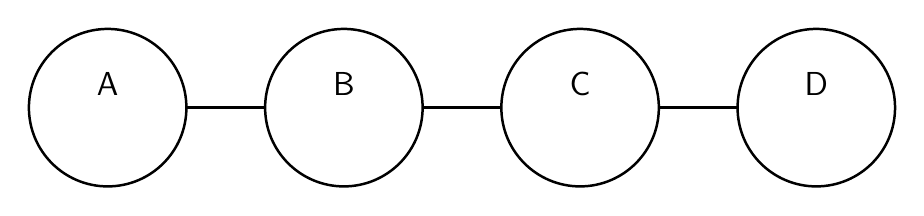
\begin{tikzpicture}[x=1cm,y=1cm,site/.style={circle,draw,line width=0.9pt,fill=white,minimum size=20mm,inner sep=0pt,font=\large},conflict/.style={line width=1.15pt}]
\coordinate (A) at (-4.5,1.5);
\coordinate (B) at (-1.5,1.5);
\coordinate (C) at (1.5,1.5);
\coordinate (D) at (4.5,1.5);
\draw[conflict] (A) -- (B);
\draw[conflict] (B) -- (C);
\draw[conflict] (C) -- (D);
\node[site] at (A) {};
\node[font=\large,yshift=3mm] at (A) {A};
\node[site] at (B) {};
\node[font=\large,yshift=3mm] at (B) {B};
\node[site] at (C) {};
\node[font=\large,yshift=3mm] at (C) {C};
\node[site] at (D) {};
\node[font=\large,yshift=3mm] at (D) {D};
\end{tikzpicture}
\end{center}
\recordline{Order:}\vspace{1cm}
\clearpage\gdef\band{Grades 4--5}
\noindent\textbf{Problem 8:} Find an order that makes the first-slot rule use four slots on this network. Find an order that uses two. Could any order use five? Explain.\par
\begin{center}
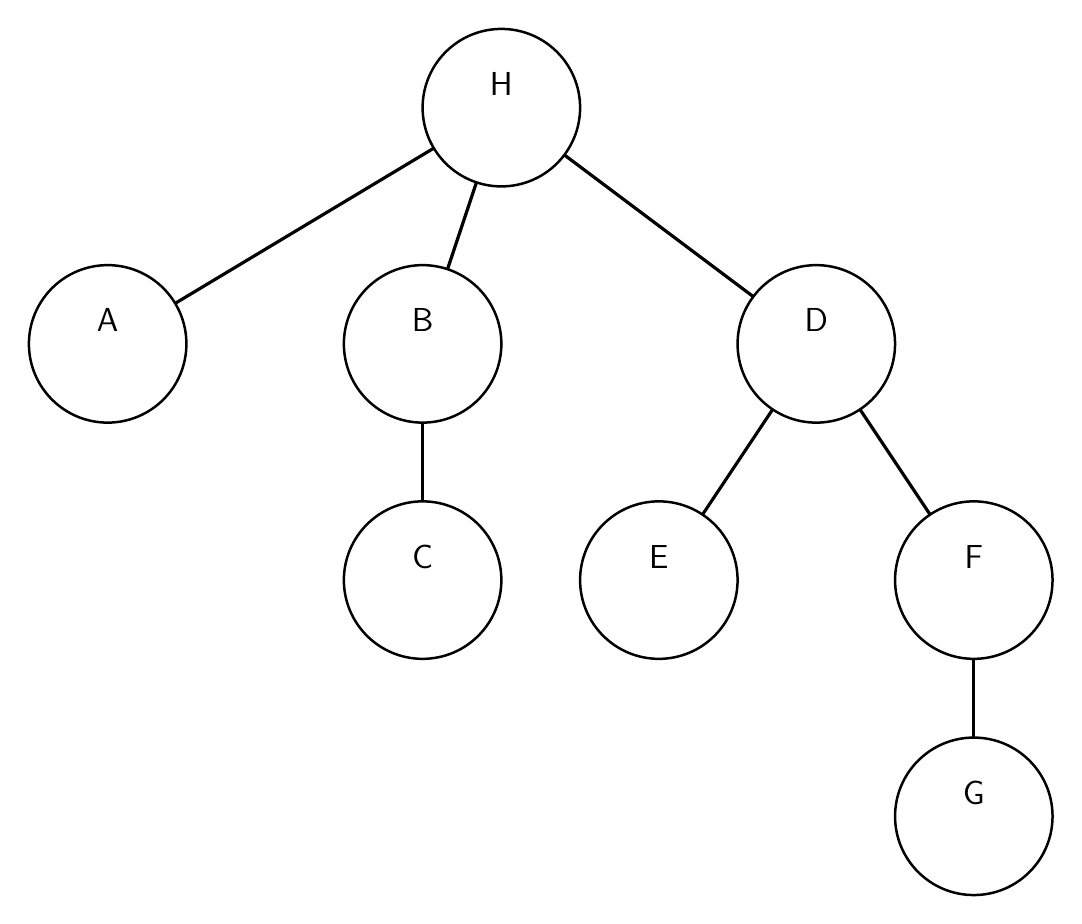
\begin{tikzpicture}[x=1cm,y=1cm,site/.style={circle,draw,line width=0.9pt,fill=white,minimum size=20mm,inner sep=0pt,font=\large},conflict/.style={line width=1.15pt}]
\coordinate (H) at (0,3);
\coordinate (A) at (-5,0);
\coordinate (B) at (-1,0);
\coordinate (D) at (4,0);
\coordinate (C) at (-1,-3);
\coordinate (E) at (2,-3);
\coordinate (F) at (6,-3);
\coordinate (G) at (6,-6);
\draw[conflict] (H) -- (A);
\draw[conflict] (H) -- (B);
\draw[conflict] (B) -- (C);
\draw[conflict] (H) -- (D);
\draw[conflict] (D) -- (E);
\draw[conflict] (D) -- (F);
\draw[conflict] (F) -- (G);
\node[site] at (H) {};
\node[font=\large,yshift=3mm] at (H) {H};
\node[site] at (A) {};
\node[font=\large,yshift=3mm] at (A) {A};
\node[site] at (B) {};
\node[font=\large,yshift=3mm] at (B) {B};
\node[site] at (D) {};
\node[font=\large,yshift=3mm] at (D) {D};
\node[site] at (C) {};
\node[font=\large,yshift=3mm] at (C) {C};
\node[site] at (E) {};
\node[font=\large,yshift=3mm] at (E) {E};
\node[site] at (F) {};
\node[font=\large,yshift=3mm] at (F) {F};
\node[site] at (G) {};
\node[font=\large,yshift=3mm] at (G) {G};
\end{tikzpicture}
\end{center}
\recordline{Four-slot order:}\recordline{Two-slot order:}\vspace{1.3cm}
\hrule\vspace{1cm}\hrule
\clearpage\gdef\band{Grades 4--5}
When counting schedules, switching slot numbers counts as a different schedule. Slots may be empty.
\begin{center}
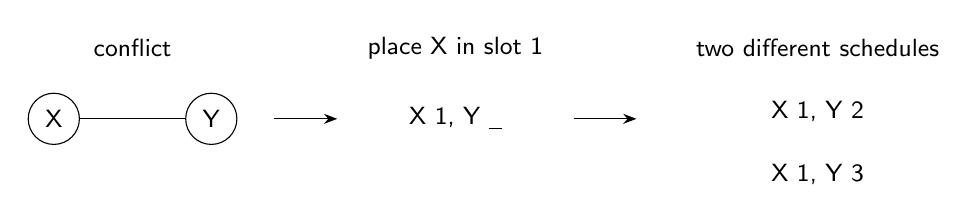
\begin{tikzpicture}[x=1cm,y=1cm,font=\small,>=Stealth]
\node at (1,1.9) {conflict};
\draw (0,1) -- (2,1);
\node[draw,circle,fill=white,minimum size=0.65cm] at (0,1) {X};
\node[draw,circle,fill=white,minimum size=0.65cm] at (2,1) {Y};
\draw[->] (2.8,1) -- (3.6,1);
\node at (5.1,1.9) {place X in slot 1};
\node at (5.1,1) {X 1, Y \underline{\phantom{3}}};
\draw[->] (6.6,1) -- (7.4,1);
\node at (9.7,1.9) {two different schedules};
\node at (9.7,1.1) {X 1, Y 2}; \node at (9.7,0.3) {X 1, Y 3};
\end{tikzpicture}
\end{center}
\noindent\textbf{Problem 9:} How many different schedules does each network have using only slots 1, 2 and 3? How many using slots 1, 2, 3 and 4? Explain how you know your count is complete.\par
\begin{center}
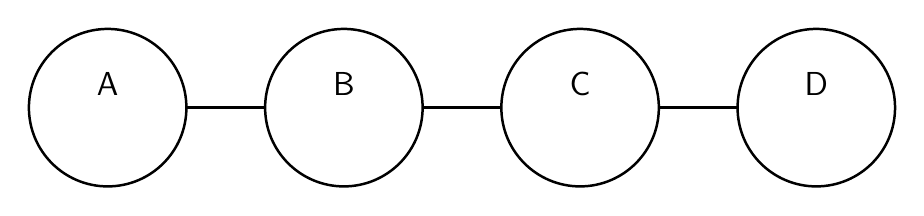
\begin{tikzpicture}[x=1cm,y=1cm,site/.style={circle,draw,line width=0.9pt,fill=white,minimum size=20mm,inner sep=0pt,font=\large},conflict/.style={line width=1.15pt}]
\coordinate (A) at (-4.5,1.5);
\coordinate (B) at (-1.5,1.5);
\coordinate (C) at (1.5,1.5);
\coordinate (D) at (4.5,1.5);
\draw[conflict] (A) -- (B);
\draw[conflict] (B) -- (C);
\draw[conflict] (C) -- (D);
\node[site] at (A) {};
\node[font=\large,yshift=3mm] at (A) {A};
\node[site] at (B) {};
\node[font=\large,yshift=3mm] at (B) {B};
\node[site] at (C) {};
\node[font=\large,yshift=3mm] at (C) {C};
\node[site] at (D) {};
\node[font=\large,yshift=3mm] at (D) {D};
\end{tikzpicture}
\end{center}
\begin{center}3 slots: \rule{1.1in}{0.4pt}\qquad 4 slots: \rule{1.1in}{0.4pt}\end{center}
\begin{center}
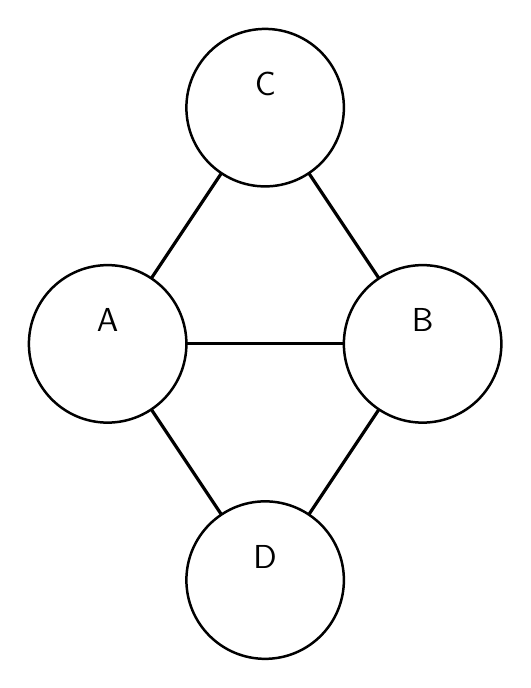
\begin{tikzpicture}[x=1cm,y=1cm,site/.style={circle,draw,line width=0.9pt,fill=white,minimum size=20mm,inner sep=0pt,font=\large},conflict/.style={line width=1.15pt}]
\coordinate (A) at (-2,0);
\coordinate (B) at (2,0);
\coordinate (C) at (0,3);
\coordinate (D) at (0,-3);
\draw[conflict] (A) -- (B);
\draw[conflict] (A) -- (C);
\draw[conflict] (B) -- (C);
\draw[conflict] (A) -- (D);
\draw[conflict] (B) -- (D);
\node[site] at (A) {};
\node[font=\large,yshift=3mm] at (A) {A};
\node[site] at (B) {};
\node[font=\large,yshift=3mm] at (B) {B};
\node[site] at (C) {};
\node[font=\large,yshift=3mm] at (C) {C};
\node[site] at (D) {};
\node[font=\large,yshift=3mm] at (D) {D};
\end{tikzpicture}
\end{center}
\begin{center}3 slots: \rule{1.1in}{0.4pt}\qquad 4 slots: \rule{1.1in}{0.4pt}\end{center}\vspace{0.7cm}
\end{document}
